% This is a template for dissertations and theses in the UCI format.
% 
% All fonts, including those for sub- and superscripts, must be 10
% points or larger.  Recommended sizes are 14-point for chapter
% headings, 12-point for the main body of text and figure/table
% titles, and 10-point for footnotes, sub- and super-scripts, and text
% in figures and tables.
%
% Notes: Add short title to figures, sections, via square brackets,
% e.g. \section[short]{long}.
%

% This block below must appear before \documentclass.
% It enables LaTeX’s PDF tagging support and sets accessibility-related PDF metadata.
\DocumentMetadata{
    tagging=on, % turns on tagged PDF output; this must be on
    pdfstandard=ua-2, % declares PDF/UA-2 as the target accessibility standard
    lang=en-US % sets the document language for PDF readers
}
% Check LaTeX Tagging Project’s guidelines for more details: https://latex3.github.io/tagging-project/documentation/usage-instructions



% ==================================================
% Start of preamble
% ==================================================
\documentclass[12pt,fleqn]{ucithesis}

% A few common packages
\usepackage{amsmath}
\usepackage{unicode-math} %Cannot be run with pdftex. only works with LuaLaTeX
%\PassOptionsToPackage{
%    showtagging=true, activate=true
%}{tagpdf}
%\usepackage{tagpdf}
\usepackage{xcolor}
\usepackage{comment}
\usepackage{amsthm}
\usepackage{array}
\usepackage{graphicx}
\usepackage[numbers]{natbib} % use [round] for parenthetical. [numbers] for numbered references.
\usepackage{bibentry}  % for putting bib entry in VITA
\usepackage{relsize}
\usepackage[titletoc]{appendix}

% Some other useful packages

%% caption and subcaption packages are not supported in tagging project yet, as of July 7, 2026. These packages do not impact accessibility, but it creates errors in Overleaf.
%\usepackage{caption}
%\usepackage{subcaption} 

\usepackage{multirow}
\usepackage{tabularx} % compatible
\usepackage{parskip} %% <-- added % compatible

% If you are unable to embed fonts such as 'Zapf Dingbats' or 'Symbol', try using raster images (.jpg or .png) instead of vector images (.pdf or .eps).
% \usepackage[T1]{fontenc} %compatible with tagging project


%% for pdf tagging
\PassOptionsToPackage{
    pdfencoding=auto,
    pdfusetitle=true,
    bookmarks=true,
    pdfpagelabels=true
}{hyperref}

% Set pdfborder to 0 0 0 to disable colored borders around PDF hyperlinks
\usepackage[plainpages=false,pdfborder={0 0 0}]{hyperref}


% Note: algorithms package has not been tested with tagging, but it is currently incompatible with the tagging project as of July 7, 2026. algorithmic package is compatible.
% Uncomment the following line to use the algorithm package,
% which provides an algorithm environment similar to figure and table
% ("\begin{algorithm}...\end{algorithm}"). A list of algorithms will
% automatically be added in the preliminary pages. Note that you
% probably want a package for the actual code to go with this (e.g.,
% algorithmic).
%\usepackage{algorithm}



% Uncomment the following to avoid "widowing", where page breaks cause
% single lines of paragraphs to float onto the next page (this is not
% a UCI requirement but more of an aesthetic choice).
%\widowpenalty=10000
%\clubpenalty=10000




% Modify or extend these at will.
\newtheorem{theorem}{\textsc{Theorem}}[chapter]
\newtheorem{definition}{\textsc{Definition}}[chapter]
\newtheorem{example}{\textsc{Example}}[chapter]

% Macros for title, author, abstract, etc.
%% This is tagged in the PDF as type "Title". This is compliant with PDF 2.0 standards. some UIs might not recognize this tag, but it's correct and all other H1s can nest under the title.
\thesistitle{Title of the Thesis}

%"Dissertation" for PhD, "Thesis" for master's
\documenttype{Dissertation}

\degreename{Doctor of Philosophy}

%NOTE: make sure your degree title is from this database: https://www.reg.uci.edu/mdsd/
\degreefield{Informatics}

% Your name as it appears on official UCI records.
\authorname{Your name}

% Use the full name of each committee member and full title 
% (e.g. Professor/Associate Professor).
\committeechair{[Assistant/Associate/Professor] First Last}
\othercommitteemembers
{
  Assistant Professor B\\
  Associate Professor C
}

\degreeyear{2026}


%NOTE: If your dissertation includes any previously published materials, including materials authored or co-authored by you, please list any additional copyrights on those materials here. Some examples are provided below.
%See the manual at https://guides.lib.uci.edu/gradmanual/copyright for more information
\copyrightdeclaration
{
    %% Optional: example with previously published materials
    Portions of Chapter 2 {\copyright} 2022 American Institute of Physics (AIP Publishing) \\
    Chapter 3 {\copyright} 2023 Josephine Bruin Publishing \\
    Photographs in Chapter 4 {\copyright} 2022 Cell Press \\
    Chapter 5  {\copyright} 2023 Scotty Highlander Publishing \\
    
    %must have this line
    All other materials {\copyright} {\Degreeyear} \Authorname
}



% The dedication page is optional
% (comment out to exclude).
% NOTE: The Dedication page is optional. Any format for justification, spacing, writing style, text size and text font is acceptable for this page; however, all text must fit within the 1-inch page margins. 
%If you choose not to include a Dedication page, delete this page. The Table of Contents will begin on page ii.
\dedications
{
  (Optional dedication page. Comment out to exclude.)
  
  To ...
}

%%%%%% Acknowledgments
%%see manual https://guides.lib.uci.edu/gradmanual/acknowledgments
\acknowledgments
{

NOTE: This page is required. In addition to general thanks or acknowledgments, the following information must be acknowledged:

If you have used copyrighted material of your own or others (e.g. if chapters of your thesis or dissertation were previously published elsewhere), you must include a statement to inform the reader that permission has been granted and state the source of the permission. See examples below.

You must acknowledge grants and other funding assistance; include grant numbers if applicable (e.g., U.S. National Science Foundation (NSF) Award \# 0123456). Please list all grant funding in a separate paragraph from your other acknowledgments. See examples below.

For more information see \url{https://guides.lib.uci.edu/gradmanual/acknowledgments}

Examples:

The text of portions of Chapter 2 of this dissertation is an adaptation of the material as it appears in Anteater, P.M., Slug, S.T.B., Triton, K., \& Bear, O.T. (2022). Chemical properties of university mascots. Chemical Physics Reviews, 1(1), 10-11, used with permission from AIP Publishing. The coauthors listed in this publication are Sammy the Banana Slug, Oski T. Bear, and King Triton. Oski T. Bear directed and supervised research which forms the basis for the dissertation.

Thank you to Cell Press for granting permission to use the copyrighted photographs in Chapter 4 of this dissertation.

Financial support was provided by the University of California, Irvine, NSF Grant DEB-8227052 and a MacArthur predoctoral fellowship in International Peace and Security granted by the Social Science Research Council.
}


% Some custom commands for your list of publications and software.
\newcommand{\mysoftentry}[3]{
    \textbf{#1} \hfill \url{#2} \\
    {\emph{#3}} \\[-6pt] %\vspace{-6pt} \\
}


%% CV
%% see the manual: https://guides.lib.uci.edu/gradmanual/vita
% Include, at minimum, a listing of your degrees and educational achievements with dates and the school where the degrees were earned. This should include the degree currently being attained. Other than that it's mostly up to you what to include here and how to format it, below is just an example.
%% NOTE: This Vita will be published permanently online. It should not be your CV or Resume that you may be using for employment. It should not contain phone numbers, email addresses, names of references or advisees, or any other information that could be considered private.
%
% CV is required for PhD theses, but not Master's
% comment out to exclude

%% REQUIRED: listing of the author's degrees and educational achievements with dates and the school where the degree was earned. include the degree currently being attained.

%% OPTIONAL: academic or professional employment, publications, presentations, patents, or other scholarly work, awards, or distinctions

%Required only for PhD dissertations.
%Brief biographical sketch of the candidate; it is not intended to be a comprehensive resume.
%Includes a listing of the author's degrees and educational achievements with dates and the school where the degree was earned.
%Includes the degree currently being attained.
%May include academic or professional employment, publications, presentations, patents, or other scholarly work, awards, or distinctions.
%Do NOT include personal information such as date or place of birth, addresses (physical or email), phone numbers, marital status, headshots, etc.

\curriculumvitae
{
\nobibliography*  % needed once, before any \bibentry call  
%%% Use the same citation style used in References

%% =============================================================
%% EDUCATION  (required)
%% =============================================================
\prelimsubsection{EDUCATION} 

\textbf{Doctor of Philosophy in Computer Science} \hfill \textbf{2012}\\
University name \hfill \emph{City, State}\\[6pt]
\textbf{Bachelor of Science in Computational Sciences}\hfill\textbf{2007}\\
Another university name \hfill \emph{City, State}


%%%NOTE: Along with education, you may include relevant professional appointments and military assignments. For non-academic positions, you can also include the range of the years appointed for the position. 

%% =============================================================
%% RESEARCH EXPERIENCE (optional)    
%% =============================================================
%\prelimsubsection{RESEARCH EXPERIENCE}
%\textbf{Graduate Research Assistant}\hfill \textbf{2007--2012} \\
%University of California, Irvine \hfill \emph{Irvine, California} \\[6pt]

%% if adding another experience, duplicate previous two lines and do not leave a new line in between the two experiences



%% =============================================================
%% TEACHING EXPERIENCE (optional)    
%% =============================================================
%\prelimsubsection{TEACHING EXPERIENCE}
%\textbf{Teaching Assistant}\hfill \textbf{2009--2010} \\
%University name \hfill \emph{City, State} \\


%% =============================================================
%% FIELD OF STUDY  (Required)
%% =============================================================
%The title of your field of study 
\prelimsubsection{FIELD OF STUDY}
Computer Science



%% =============================================================
%% PUBLICATIONS  (OPTIONAL)
%% =============================================================
%%% Use the same citation style used in References
%% List of formatted publication, in alphabetical order, following standard citations requirements.
%% NOTE: You may include any of your publications (e.g. papers published as part of a conference, while completing your Bachelor’s degree, etc.) 
\prelimsubsection{PUBLICATIONS}

\bibentry{latex_tagging_status}.


%% feel welcome to use bibentry or to format the citations manually using LaTeX format. Example below. 

U. Libraries. (2026). Thesis / Dissertation Formatting Manual (2026).



%% =============================================================
%% SOFTWARE  (OPTIONAL)
%% =============================================================
%\vspace{10pt}
%\prelimsubsection{SOFTWARE}
%\mysoftentry{Magical tool}{http://your.url.here/}{}


}

% The abstract was previously limited to a maximum of 350 words, 
% but the UCI manual at https://etd.lib.uci.edu/electronic/td2e#2.2.1.
% currently does not indicate that there is any word limit for the abstract
%as of April 2026 NOTE: The text must be double-spaced. It is recommended that the text be around 350 words in length. Use indent or flush left at the beginning of paragraphs, depending on the style manual you are following. Include a short statement of the problem you studied, a brief exposition of the methods and procedures employed in gathering the data, and a summary of your findings. No graphs, charts, or tables may be included.
\thesisabstract
{
  The abstract of your contribution goes here.

  NOTE: The text must be double-spaced. It is recommended that the text be around 350 words in length. Use indent or flush left at the beginning of paragraphs, depending on the style manual you are following. Include a short statement of the problem you studied, a brief exposition of the methods and procedures employed in gathering the data, and a summary of your findings. No graphs, charts, or tables may be included.
}


%%% Local Variables: ***
%%% mode: latex ***
%%% TeX-master: "thesis.tex" ***
%%% End: ***


% Add PDF document info fields
\hypersetup{
	pdftitle={\Thesistitle},
	pdfauthor={\Authorname},
	pdfsubject={\Degreefield},
}

% Uncomment the following to have numbered subsubsections (by default numbering goes only to subsections (3.1.1)).
%\setcounter{secnumdepth}{4} % makes it go to the paragraph heading, like 3.1.1.1.1
%\setcounter{secnumdepth}{3} % makes it number up to the subsubsection 3.1.1.1


% Set this to only select a subset of the includes directives below.
% Very handy to speed up compilation if you're working on a certain
% part of your thesis. It conserves page numbers, references, etc.
% even for non-included files.
%\includeonly{chapter1}

% ========================================
% End of preamble; Start of document body
% =========================================
\begin{document}


% Preliminary pages are always loaded (TOC, CV, etc.)
\preliminarypages


% NOTE: All text is double spaced. All text and hyperlinks must be the same font, same font size (10-12pt), and in black colored text. All text must be the same justification, like left justified or fully justified. All text, figures/tables, captions, and equations must fit within the 1-inch margins.
% After your Abstract, the page numbers reset at 1, 2, 3.


% Include the different components of your thesis, in separate files.
% Using \include allows you to set \includeonly above.
\chapter{Introduction}
% the word introduction should be a H1 or H2?
% the "\section{Background}" is autotagged as H2


This is an example using the \LaTeX{} template for UCI theses and
dissertation documents. 

NOTE: All text is double spaced. All text and hyperlinks must be the same font, same font size (10-12pt), and in black colored text. All text must be the same justification, like left justified or fully justified. All text, figures/tables, captions, and equations must fit within the 1-inch margins. 
After your Abstract, the page numbers reset at 1, 2, 3.


See the UCI Thesis/Dissertation Manual for more information \cite{uci_thesis_manual}.


\section{\LaTeX{} Tagging Project}

This template uses automatic tagging support from the \LaTeX{} Tagging project \cite{latex_tagging_instructions}, an ongoing effort by the \LaTeX{} Project to make \LaTeX{}-generated PDFs accessible by default. PDF tags describe the logical structure of the document (e.g., headings, lists, tables, figures, links, etc.), which allows assistive technologies and other tools to interpret the content meaningfully, rather than treating the document as a flat stream of text. The project is building tagging support directly into the \LaTeX{} kernel and core packages, so that much of the document structure can be tagged automatically. Authors still need to provide semantic and accessibility information where needed. See \autoref{sec:chapter-2} for details.

For auto tagging to work correctly, use \TeX{} Live 2025 or newer. For the compiler, Lua\LaTeX{} is recommended, as it has the most complete tagging support. pdf\LaTeX{} also works with auto tagging but has some limitations. In Overleaf, you can configure the \TeX{} Live version and compiler under Settings \textrightarrow\ Compiler.

Note that while \LaTeX{} tagging support is increasingly capable, the project is still under active development. Most commonly used packages are compatible with auto-tagging, but not all. Before adding a new package, check the Tagging Status of \LaTeX{} Packages and Classes \cite{latex_tagging_status}, which is updated as support evolves.

% previous latex template \cite{uci-thesis-latex}


%%% Local Variables: ***
%%% mode: latex ***
%%% TeX-master: "thesis.tex" ***
%%% End: ***


\chapter{Accessibility Information} \label{sec:chapter-2}

Accessible documents enable readers who use assistive technologies—such as screen readers, braille displays, or text-to-speech tools—to read and navigate content. This supports people with disabilities, including people who are blind, have low vision, or have other print disabilities. Accessible documents also benefit all readers: well-structured documents are easier to navigate, reflow better on small screens, and can be more reliably parsed by search engines and automated tools.

While this template provides auto-tagging support, it does not make a document fully accessible by itself. Authors still need to use semantic \LaTeX{} commands and provide the information that cannot be inferred automatically, such as alt text for figures and table headers. The following sections include guidance on making content accessible.

\section{Headings}

Use \LaTeX{} sectioning commands to create headings, so that they can be automatically tagged with the correct heading levels in the PDF and displayed by PDF viewers as a document outline.

\begin{itemize}
    \item \verb|\thesistitle| creates the top level tag Title
    \item \verb|\chapter| creates a level 1 heading (H1)
    \item \verb|\section| creates a H2
    \item \verb|\subsection| creates a H3
    \item \verb|\subsubsection| creates a H4
    \item \verb|\paragraph| creates a H5
    \item \verb|\subparagraph| creates a H6
\end{itemize}

Make sure to use heading levels in order and avoid skipping heading levels.

\section{Figures}

NOTE: Figure captions go below figures and must use the “Caption” style in order to auto-populate a List of Figures. 

NOTE: All images must include alt-text. 
%To insert alt-text to images, hover over the image > right click > view alt text > input the description for the image



\begin{figure}[ht]
    \centering
    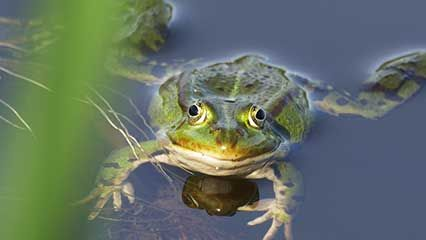
\includegraphics[alt={a green frog is laying in a pond}, width=0.7\linewidth]{figures/frog.jpg}
    \caption{A frog on a log}
    \label{fig:frog}
\end{figure}

\TeX{} Live 2025 or newer versions have auto tagging for figures. However, alt text still needs to be added manually in the \LaTeX{} source; it is not automatically generated when a figure is created. 

To insert alt text, add the “\verb|alt|” key inside the \verb|\includegraphics| command, as in \texttt{alt=\{a green frog is lying in a pond\}}. See the \LaTeX{} code example in \autoref{fig:frog}. This alt text will then be automatically included in the PDF tags.

In general, useful alt text should begin with a high-level summary of the figure, followed by as much relevant detail as possible to help readers understand the figure’s meaning or purpose. For more detailed guidance, see SIGACCESS’s guide \cite{trewin2019} on describing figures.


\begin{figure}[ht]
    \centering
    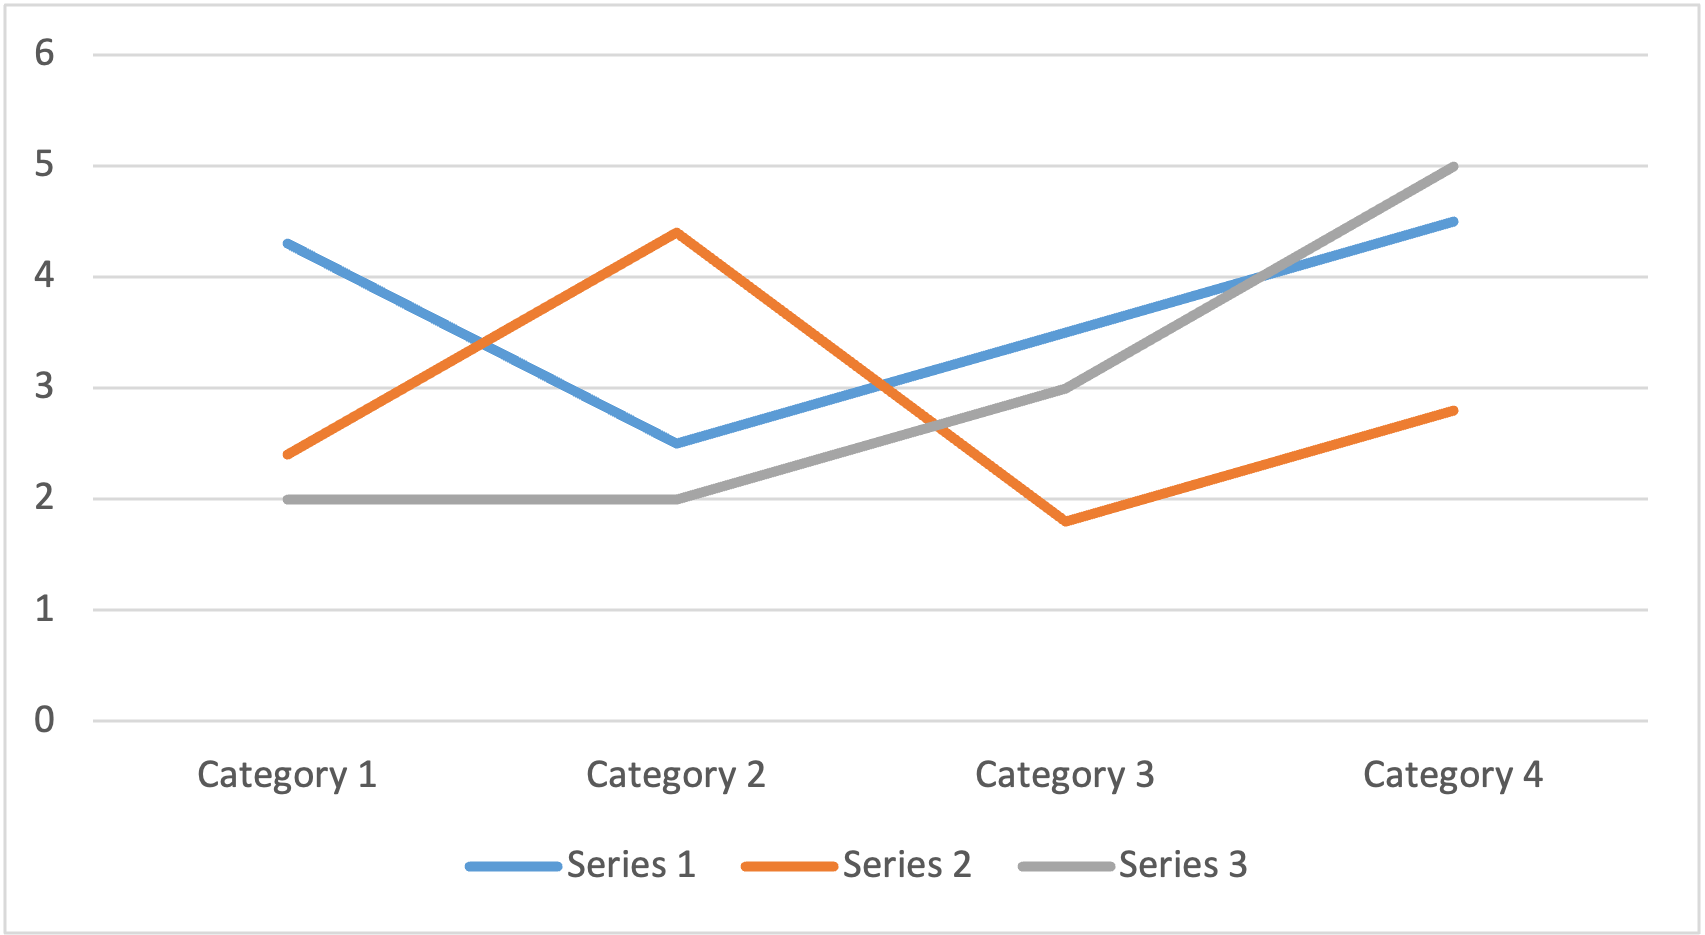
\includegraphics[alt={Line chart comparing values for 3 series across 4 categories. x-axis shows Categories 1 through 4, y-axis ranges from 0 to 6. Overall, Series 1 and Series 3 end higher than they begin, while Series 2 rises and falls. Series 1 decreases at first, then increases. Series 2 peaks in Category 2 and reaches its lowest value in Category 3. Series 3 stays flat at first, then increases. Approximate values from Categories 1 to 4 are: 4.3, 2.5, 3.4, 4.5 for Series 1; 2.4, 4.4, 1.8, and 2.8 for Series 2; 2.0, 2.0, 3.0, and 5.0 for Series 3.}, width=0.7\linewidth]{figures/chart_template.png}
    \caption{Example chart}
    \label{fig:chart}
\end{figure}



\autoref{fig:sourcecode} is just for illustration purposes, as is \autoref{tab:coordinates}. Note that these figures and tables are made of text and are highlightable. No images of text. 


\begin{figure}[ht]
\begin{verbatim}
#include <iostream>
int main(int argc, char** argv) {
  std::cout << "Hello World." << std::endl;
  return 0;
}
\end{verbatim}
  \caption{Example source code.}
  \label{fig:sourcecode}
\end{figure}






\section{Tables}


%NOTE: Table captions go above tables and must use the “Caption” style in order to auto-populate a List of Tables. % from the Word template
NOTE: Table captions go above tables and auto-populate a List of Tables. 
If any caption is more than four lines, all captions must be single spaced. In general, we recommend single spacing captions. 

Tables should be created as real \LaTeX{} tables using the \verb|tabular|, \verb|tabularx|, or similar table environments, rather than inserted as images of tables.

Each table should have its header row defined. Typically, the header is the first row. To mark the first row as the header row, add \verb|\tagpdfsetup{table/header-rows={1}}| above the table environment (before \verb|\begin{table}|). See the \LaTeX{} code example in \autoref{tab:coordinates}.
If the table has multiple header rows, list all header row numbers. For example, if rows 1 and 2 are both header rows, use \verb|\tagpdfsetup{table/header-rows={1,2}}|.


\tagpdfsetup{table/header-rows={1}}
\begin{table}[h]
  \centering
  \caption{Example coordinates.}
  \begin{tabular}{|rr|r|}
    \hline
    $x$ & $y$ & $z$ \\
    \hline
    14 & 12 & -2 \\
    0 & 33 & -25 \\
    -3 & 11 & 22 \\
    4 & 4 & 6 \\
    \hline
  \end{tabular}
  \label{tab:coordinates}
\end{table}


\tagpdfsetup{table/header-rows={1}}
\begin{table}[htbp]
\centering
\caption{City or Town Distance Matrix}
\label{tab:city_distance}
\begin{tabularx}{\textwidth}{|>{\raggedright\arraybackslash}p{3cm}|*{5}{>{\raggedright\arraybackslash}X|}}
\hline
\textbf{City or Town} & \textbf{Point A} & \textbf{Point B} & \textbf{Point C} & \textbf{Point D} & \textbf{Point E} \\ \hline
Point A & --- &     &     &     &     \\ \hline
Point B & 87  & --- &     &     &     \\ \hline
Point C & 64  & 56  & --- &     &     \\ \hline
Point D & 37  & 32  & 91  & --- &     \\ \hline
Point E & 93  & 35  & 54  & 43  & --- \\ \hline
\end{tabularx}
\end{table}



\section{Math Equations}

\TeX{} Live 2025 can auto tag math equations as “Formula” and attaches the corresponding MathML to the PDF. Compatible PDF viewers, such as Adobe Acrobat Pro, can use this MathML to make equations available to assistive technologies. The generated MathML can be found in the PDF’s attachments panel using Acrobat Pro.

$$ \int_1^{12} \frac{x^2}{5 - \sqrt{5}} \,dx $$

We can also try labeling equations.
\begin{equation}\label{eqn:einstein}
E=mc^2
\end{equation}
Then we can refer to \autoref{eqn:einstein}.


% ... and so on


% This command ensures the bibliography line of the Table of Contents shows the correct page number.
\clearpage


% Choose what to call the bibliography section: "Bibliography" or "References".
% Default is "Bibliography".        
\bibliographyname{Bibliography} 

% Single space each entry.
\begin{spacing}{1}    

% References should be formatted in style most common in discipline
%Work with your faculty advisor to determine your citation style (Chicago, APA, MLA.) – any style is accepted, just be consistent.
% abbrv is a suggestion.
% ACM-Reference-Format is an option for scholars who publish in ACM venues; that reference-format file is available separately (not bundled with this template). Other venues may use other formats.
\bibliographystyle{abbrv}
\bibliography{references}
\end{spacing}    
% You may have one all-encompassing Reference section at the end of your paper, or individual Reference sections at the end of each chapter. Choose one.
% If any chapter of your dissertation is a reproduction of a previously published article, that article must be included in the Reference section.


% The Thesis Manual says not to include appendix figures and tables in the List of Figures and Tables, respectively, so these commands from the caption package turn it off from this point onwards. If needed, it can be re-enabled later (using list=yes argument).
%\captionsetup[figure]{list=no}
%\captionsetup[table]{list=no}



%% Overleaf tagging note: putting these here causes an issue with how the captions interact with the LOF/LOT contents pages. causes warnings
% The warnings come from the caption package's \addcontentsline{lof/lot} call interacting with tagpdf 0.99q



% If you have an appendix, it should come after the references.
\appendix

\chapter{Appendix Title}

% Appendix sections, subsections etc should not appear in the table of contents. So set tocdepth to 0 and set it back to 2 at the end. Do this for each appendix.
\addtocontents{toc}{\protect\setcounter{tocdepth}{0}}

Supplementary material goes here. 

%Any tables or figures in the appendix do not appear in the List of Tables or the List of Figures.

\section{Example Section}

\subsection{Example Sub Section}



\addtocontents{toc}{\protect\setcounter{tocdepth}{2}}





\end{document}
% =========================================
% End of document body
% =========================================